El objetivo de este capítulo es demostrar las partes importantes o de interés de la implementación y como se ha logrado la realización de lo mencionado en capítulos anteriores.

\section{El monorepo del proyecto}

Una de las cosas fundamentales a la hora de crear este proyecto era conseguir dividir el proyecto en varias secciones sin dificultar el trabajar con ellas a la vez. Es por esto que se decidió usar un monorepo para guardar el proyecto y aprovechar de ciertas herramientas para facilitar su uso. Como herramienta principal para gestionar el monorepo se decidió usar \verb|turborepo|\cite{turborepo}, debido a que es uno de las más populares y de los que más rendimiento tienen a la hora de construir las aplicaciones. Además de usar turborepo, se decidió aprovechar una de las opciones que trae el gestor de paquetes \verb|pnpm|\cite{pnpm}, los \verb|worspaces|\cite{pnpm-workspaces}, la cual permite unir varios proyectos dentro del mismo repositorio y compartir las dependencias entre ellos. Por último, se utilizó la herramienta \verb|changesets|\cite{changesets} para el control de versiones de los diferentes paquetes y proyectos del monorepo.

\section{El inicializador de {\tt adastra}}

Como se dijo anteriormente en el apartado de diseño se ha creado un paquete llamado \verb|create-adastra-lms|, que sirve como punto de inicio para crear un proyecto con AdAstra. La función principal de este paquete se muestra en la figura \ref{fig:adastraCreateMain}. Lo primero que se realiza es la extracción de los argumentos pasados al programa, para luego crear un objeto \verb|context|, que proporciona los datos que necesitará la aplicación, en función de estos argumentos. En caso de que se haya pasado como argumento una \textit{flag} de ayuda, como \verb|-h| o \verb|--help|, se mostrará el menú de ayuda como resultado, se puede ver en la figura \ref{fig:adastraCreateHelp}. Para finalizar, se ejecutarán los diferentes pasos de la ejecución, encapsulados dentro de un array, que en este caso se tratan de diferentes funciones asíncronas que se llamarán una después de otra. Para facilitar el proceso de creación de este paquete se ha usado, una librería del framework de \verb|Astro|\cite{astro} llamada \verb|@astrojs/cli-kit|\cite{astro-cli} que suministra de diferentes utilidades que sirven para facilitar la creación de un programa de cli, como la petición de un prompt o las personalización de los mensajes. 

\begin{figure}
    \begin{lstlisting}[language=Javascript]
        export const main = async () => {
          const clearArgv = process.argv.slice(2).filter((arg) => arg !== "--");
          const context = getContext(clearArgv);
          if (context.help) return help();
        
          const steps = [projectName, template, dependecies, git, next];
        
          for (const step of steps) {
            await step(context);
          }
        
          exit();
        };
    \end{lstlisting}
    \caption{Función principal de create-adastra-lms}
    \label{fig:adastraCreateMain}
\end{figure}

\begin{figure}
    \centering
    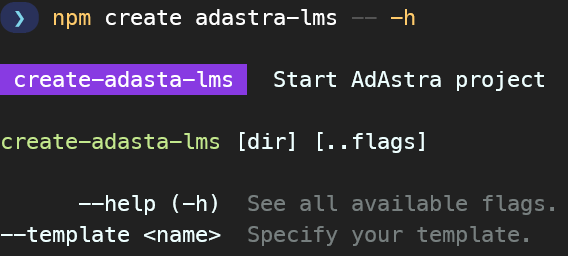
\includegraphics{images/adastraHelp.png}
    \caption{Salida del flag de ayuda de create-adastra-lms}
    \label{fig:adastraCreateHelp}
\end{figure}

Ahora vamos a explicar en más profundidad cada parte.

\subsection{La función {\tt getContext}}
Está función se encarga de extraer los valores de los argumentos y convertirlo a los datos deseados a través de la librería \verb|arg|\cite{arg}. Tras se usará el primer parametro pasado como \verb|cwd| y posible nombre del proyecto a crear y se usa la función \verb|detectPackageManager| de la librería \verb|which-pm-runs|\cite{which-pm-runs} para detectar cual manejador de paquetes se está usando y guardar este dato. Con todo esto se construirá un objeto \verb|context| que será el resultado de la función. En la figura \ref{fig:adastraCreateContext} se puede ver en más profundidad esta función.

\begin{figure}
    \begin{lstlisting}[language=Javascript]
        export interface Context {
          help: boolean;
          prompt: typeof prompt;
          cwd: string;
          pkgManager: string;
          projectName?: string;
          template?: string;
          install?: boolean;
          exit(code: number): never;
        }

        export const getContext = (argv: string[]): Context => {
          const flags = arg(
            {
              "--help": Boolean,
              "--template": String,
        
              "-h": "--help",
            },
            { argv, permissive: true }
          );
        
          const pkgManager = detectPackageManager()?.name ?? "npm";
          let cwd = flags["_"][0];
          let { "--help": help = false, "--template": template } = flags;
          let projectName = cwd;
        
          const context: Context = {
            help,
            prompt,
            pkgManager,
            projectName,
            template,
            cwd,
            exit: (code) => {
              process.exit(code);
            },
          };
          return context;
        };
    \end{lstlisting}
    \caption{Función getContext de create-adastra-lms}
    \label{fig:adastraCreateContext}
\end{figure}

\subsection{El paso {\tt projectName}}

Dentro de este paso lo primero que se comprueba es que en caso de si se ha pasado un \verb|cwd| como argumento, este sea valido para usar y este vació. En caso de que la comprobación sea fallida, el programa pedirá al usuario que la ubicación deseada a usar, comprobando que esta sea valida, esta ubicación será el cwd a usar para el proyecto. Tras esto, tanto si el cwd fue valido o no, se extraerá un nombre valido para el proyecto, con la función \verb|toValidName|, que corrigue a un nombre valido el string que se le pase. En la figura \ref{fig:adastraCreateProjectName} se ve las partes importantes del código de este paso.

\begin{figure}
    \begin{lstlisting}[language=Javascript]
        const checkCwd = async (cwd: string | undefined) => {
          const empty = cwd && isEmpty(cwd);
          if (empty) {
            log("");
            await info(
              "dir",
              `Using ${color.reset(cwd)}${color.dim(" as project directory")}`
            );
          }
        
          return empty;
        };
        
        export const projectName = async (context: Context) => {
          await checkCwd(context.cwd);
        
          if (!context.cwd || !isEmpty(context.cwd)) {
            if (!isEmpty(context.cwd)) {
              await info(
                "Hmm...",
                `${color.reset(`"${context.cwd}"`)}${color.dim(` is not empty!`)}`
              );
            }
        
            const { name } = await context.prompt({
              name: "name",
              type: "text",
              label: title("dir"),
              message: "Where should we create your new project?",
              initial: `./${generateProjectName()}`,
            });
        
            context.cwd = name!;
            context.projectName = toValidName(name!);
          } else {
            let name = context.cwd;
            context.projectName = toValidName(extractName(name));
          }
        
        };
    \end{lstlisting}
    \caption{Paso projectName de create-adastra-lms}
    \label{fig:adastraCreateProjectName}
\end{figure}

\subsection{El paso {\tt template}}

Este es uno de los pasos más importantes y es que este se encarga de descargar y preparar la \textit{template}, de la cual hablaremos después, a usar para el proyecto. Lo primero que se hace es comprobar si se ha pasado una template como argumento, en caso negativo, se le pide al usuario de entre una lista de templates que escoja la deseada. Tras saber que template se va a querer usar, se empezará el proceso de copia de esta en el que se llamará a la función \verb|copyTemplate| En la figura \ref{fig:adastraCreateTemplate} se puede el código de este paso. Dentro de esta primero se intentará descargar la template deseada con la librería \verb|giget|\cite{giget}, que facilita la descarga de proyectos de GitHub a través de un programa de Javascript, a una carpeta llamada \verb|.adastra|, que guardara toda la lógica y funcionamiento del LMS. En caso de que la descarga de un error el programa se parará y mostrará el error. Si todo va bien lo siguiente que se hará es mover el archivo \verb|package.json| que trae la template, que en este caso esta dentro de \verb|.adastra/package.json| a la carpeta principal del proyecto para usarlo como el archivo \verb|package.json| de este proyecto. Tras haber reubicado este archivo se pasará a realizar ciertos cambios a este como cambiar el nombre al del proyecto y cambiar los \verb|scripts| de npm para que seán los siguientes:
\begin{verbatim}
    scripts: {
        dev: 'astro dev --root "./.adastra"',
        build: 'astro build --root "./.adastra"',
    }
\end{verbatim}
Con estos scripts se define que se deberá usar la carpeta \verb|.adastra| como la carpeta principal a usar por el framework Astro, esto se debe a que para simplificar la experiencia del usuario se decide ocultar la lógica principal del programa de Astro creado en la carpeta \verb|.adastra|, por lo que se deberá usar esa carpeta como \verb|root| del proyecto y no la carpeta principal como normalmente haría el framework. Tras esto se moverá también el archivo \verb|.gitignore| de la template a la carpeta principal, se creará el archivo .env  para que el usuario pueda introducir la variable de entorno \verb|GITHUB_SECRET| en local y el archivo \verb|adastra.config.mjs| con la configuración necesaria del proyecto. Por último se crearán link simbólicos que permitan modificar el contenido del proyecto de Astro dentro de \verb|.adastra|, pero sin tener que entrar dentro de la lógica de este. Estos serían los siguientes:

\begin{itemize}
    \item Se vinculará el archivo \verb|.env| creado en la carpeta principal del proyecto con uno dentro de la carpeta \verb|.adastra|, esto es necesario ya que al definir anteriormente que el root a usar a la hora de iniciar el framework de astro fuera la carpeta \verb|.adastra| de normal mirará ahi si se encuentra el archivo \verb|.env| y no fuera de esta.
    \item Se vinculará las carpetas \verb|classes|, \verb|labs| y \verb|subjects| con las carpetas con sus respectivas contra partes dentro de la carpeta \verb|content| del proyecto de Astro, donde se guarda los contenido markdown a usar. En este caso serían:
    \begin{verbatim}
        .adastra/src/content/docs/1-activities/1-classes
        .adastra/src/content/docs/1-activities/2-labs
        .adastra/src/content/docs/1-activities/3-subjects
    \end{verbatim}
\end{itemize}

En la figura \ref{fig:adastraCreateTemplateCopy} se puede ver mejor la función \verb|copyTemplate|.

\begin{figure}
    \begin{lstlisting}[language=Javascript]
        export const template = async (context: Context) => {
          if (!context.template) {
            const { template: tmpl } = await context.prompt({
              name: "template",
              type: "select",
              label: title("tmpl"),
              message: "How would you like to start your new project?",
              initial: "basic",
              choices: [
                {
                  value: "basic",
                  label: "Basic LMS",
                  hint: "(recommended)",
                },
              ],
            });
            context.template = tmpl;
          } else {
            await info(
              "tmpl",
              `Using ${color.reset(context.template)}${color.dim(
                " as project template"
              )}`
            );
          }
        
          await spinner({
            start: "Template copying...",
            end: "Template copied",
            while: () =>
              copyTemplate(context.template!, context as Context).catch((e) => {
                if (e instanceof Error) {
                  error("error", e.message);
                  process.exit(1);
                } else {
                  error("error", "Unable to clone template.");
                  process.exit(1);
                }
              }),
          });
        };
    \end{lstlisting}
    \caption{Paso template de create-adastra-lms}
    \label{fig:adastraCreateTemplate}
\end{figure}

\begin{figure}
    \begin{lstlisting}[language=Javascript]
        const copyTemplate = async (template: string, context: Context) => {
          const templateTarget = `.../${template}`;
        
          try {
            await downloadTemplate(templateTarget, {
              force: true, provider: "github", cwd: context.cwd, dir: "./.adastra"
            });
          } catch (err: any) {
            throw new Error(err.message);
          }
        
          fs.renameSync(`${context.cwd}/.adastra/package.json`,`${context.cwd}/package.json`);
        
          const updateFiles = Object.entries(FILES_TO_UPDATE).map(
            async ([file, update]) => {
              const fileLoc = path.resolve(path.join(context.cwd, file));
              if (fs.existsSync(fileLoc)) {
                return update(fileLoc, {
                  name: context.projectName!,
                  scripts: {
                    dev: 'astro dev --root "./.adastra"',
                    build: 'astro build --root "./.adastra"',
                  },
                });
              }
            }
          );
        
          await Promise.all([...updateFiles]);
        
          fs.renameSync(`${context.cwd}/.adastra/.gitignore`,`${context.cwd}/.gitignore`);
          fs.writeFileSync(`${context.cwd}/.env`, "GITHUB_SECRET=\n");
        
          fs.writeFileSync(
            `${context.cwd}/adastra.config.mjs`,
            `export const tailwindConfig = { ... };
        
        export const organizationInfo = { ... };
        `);
        
          fs.symlinkSync(`../.env`, `${context.cwd}/.adastra/.env`, "file");
          symlinkDir(`${context.cwd}/.adastra/public`, `${context.cwd}/public`);
          symlinkDir(`${context.cwd}/.adastra/src/content/docs/1-activities/1-classes`,`${context.cwd}/classes`);
          ...
        };
    \end{lstlisting}
    \caption{Función copyTemplate simplificada del paso template de create-adastra-lms}
    \label{fig:adastraCreateTemplateCopy}
\end{figure}

\subsection{El paso {\tt dependencies}}

En el siguiente paso de la ejecución se le preguntará al usuario si se querrá instalar las dependencias ahora, sino se le notificará que deberá hacerlo más tarde. Si se acepta instalar, el programa usará la librería \verb|execa|\cite{execa}, que facilita la ejecución de otros procesos, para llamar el comando \verb|install| junto con el manejador de paquetes, que anteriormente se había detectado y guardado en \verb|context|. En la figura \ref{fig:adastraCreateDependencies} se puede ver el codigo de esto.

\begin{figure}
    \begin{lstlisting}[language=Javascript]
        const install = async ({
          pkgManager,
          cwd,
        }: {
          pkgManager: string;
          cwd: string;
        }) => {
          const installExec = execa(pkgManager, ["install"], { cwd });
          return new Promise<void>((resolve, reject) => {
            setTimeout(() => reject(`Request timed out after one minute`), 300_000);
            installExec.on("error", (e) => reject(e));
            installExec.on("close", () => resolve());
          });
        };
        
        export const dependecies = async (context: Context) => {
          const { deps } = await context.prompt({
            name: "deps",
            type: "confirm",
            label: title("deps"),
            message: `Install dependencies?`,
            hint: "recommended",
            initial: true,
          });
          context.install = deps;
        
          if (!deps)
            return await info(
              "No problem!",
              "Remember to install dependencies after setup."
            );
        
          await spinner({
            start: `Dependencies installing with ${context.pkgManager}...`,
            end: "Dependencies installed",
            while: () =>
              install({ pkgManager: context.pkgManager, cwd: context.cwd }).catch(
                (e) => {
                  error("error", e);
                  process.exit(1);
                }
              ),
          });
        };
    \end{lstlisting}
    \caption{Paso dependencies de create-adastra-lms}
    \label{fig:adastraCreateDependencies}
\end{figure}

\subsection{El paso {\tt git}}

Este paso es parecido al anterior, solo que en este caso se pregunta si se quiere iniciar un proyecto de \verb|git|\cite{git}, en caso de que no existiera previamente. En caso afirmativo, se usará \verb|execa| al igual que antes para llamar en este caso los siguientes comandos de git que permiten empezar un repositorio:
\begin{verbatim}
    git init
    git add -A
    git commit -m Initial commit from AdAstra 
\end{verbatim}

En la figura \ref{fig:adastraCreateGit} se puede visualizar el código de este paso.

\begin{figure}
    \begin{lstlisting}[language=Javascript]
        const init = async ({ cwd }: { cwd: string }) => {
          try {
            await execa("git", ["init"], { cwd, stdio: "ignore" });
            await execa("git", ["add", "-A"], { cwd, stdio: "ignore" });
            await execa(
              "git",
              [
                "commit",
                "-m",
                "Initial commit from AdAstra",
              ],
              { cwd, stdio: "ignore" }
            );
          } catch (e) {
            console.error(e)
          }
        };
        
        export const git = async (context: Context) => {
          if (fs.existsSync(path.join(context.cwd, ".git")))
            return await info("Nice!", `Git has already been initialized`);
        
          const { git } = await context.prompt({
            name: "git",
            type: "confirm",
            label: title("git"),
            message: `Initialize a new git repository?`,
            hint: "optional",
            initial: true,
          });
        
          if (!git)
            return await info(
              "Sounds good!",
              `You can always run ${color.reset("git init")}${color.dim(" manually.")}`
            );
        
          await spinner({
            start: "Git initializing...",
            end: "Git initialized",
            while: () =>
              init({ cwd: context.cwd }).catch((e) => {
                error("error", e);
                process.exit(1);
              }),
          });
        };
    \end{lstlisting}
    \caption{Paso git de create-adastra-lms}
    \label{fig:adastraCreateGit}
\end{figure}




% \begin{figure}[H]
%     \centering
%     \makebox[\textwidth][c]{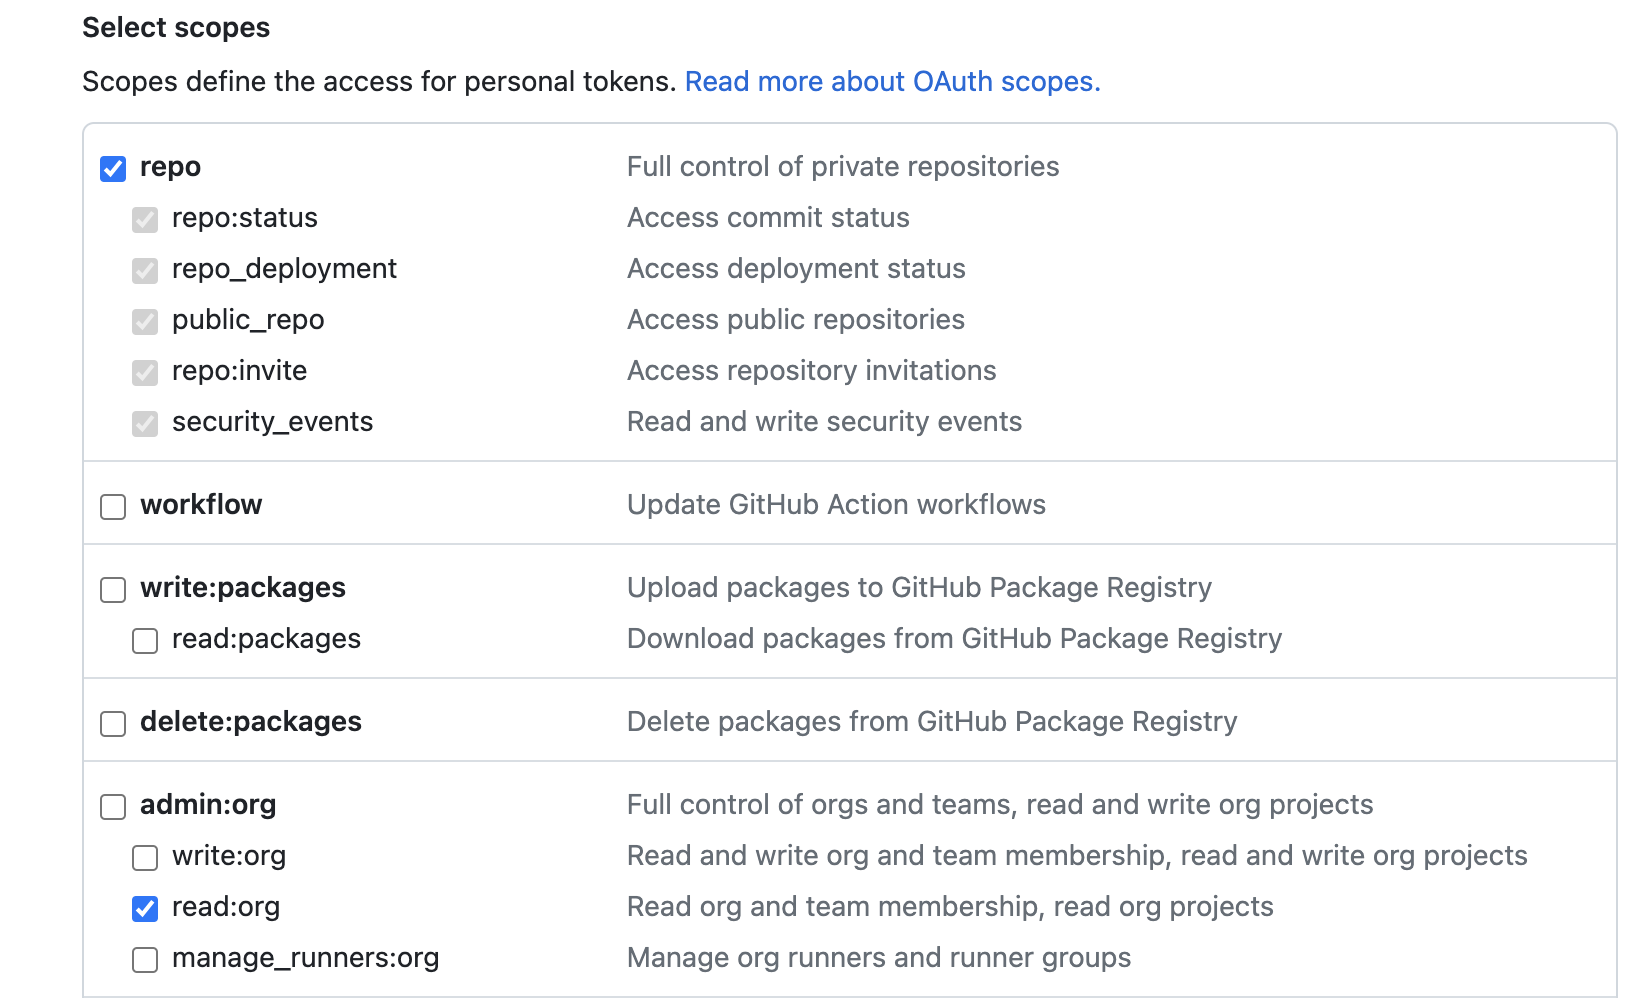
\includegraphics[width=\textwidth]{images/scopes.png}}
%     \caption{Scopes para el token GITHUB\_SECRET}
%     \label{fig:scopes}
% \end{figure}


% \section{El controlador}
% Como se ha comentado en capítulos anteriores, la mayoría de comandos se aprovecha de los comandos ya proporcionados por \verb|gh|. Como es el caso de \verb|gh edu install|. Después de determinar si la extensión es \emph{first-party} o \emph{third-party} (extensión independiente de la organización \verb|gh-cli-for-education|), se obtiene la dirección del repositorio de la extensión, se invoca \verb|gh extension install| y se añade a \verb|data.json|.

% \begin{figure}[H]
%     \centering
%     \makebox[\textwidth][c]{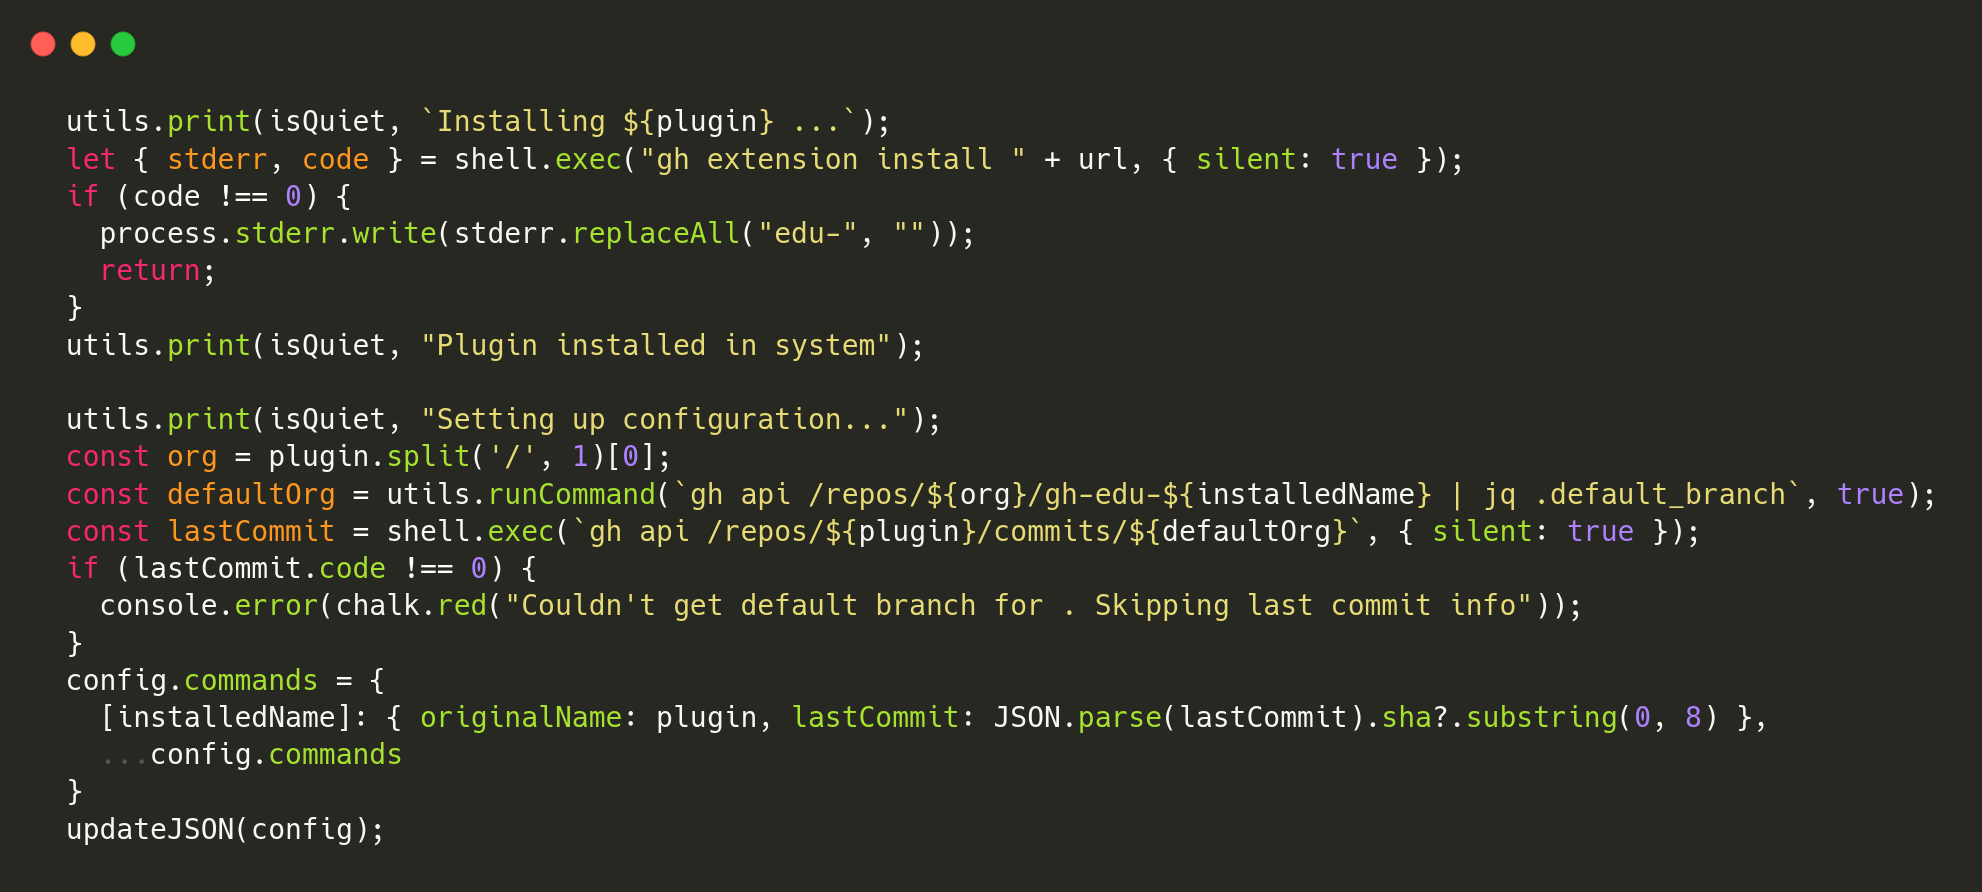
\includegraphics[width=\textwidth]{images/installCode.png}}
%     \caption{Implementación. Código para instalar extensiones}
%     \label{fig:installCode}
% \end{figure}

% En la figura \ref{fig:installCode} vemos que después de instalar la extensión, hacemos una llamada \emph{API REST} para saber cuál es la rama por defecto. Al tener esta información, podemos buscar cuál es el \gls{hash} del último \emph{commit}, para actualizar el campo \verb|lastCommit|.

% \emph{Nota: utils.print() es una función muy simple para determinar si el mensaje debería imprimirse o no, dependiendo del valor del flag --quiet}.

% Para que \verb|commander| acepte únicamente las extensiones instaladas, se ha escrito el siguiente código (figura \ref{fig:addThirdParty}):

% \begin{figure}[H]
%     \centering
%     \makebox[\textwidth][c]{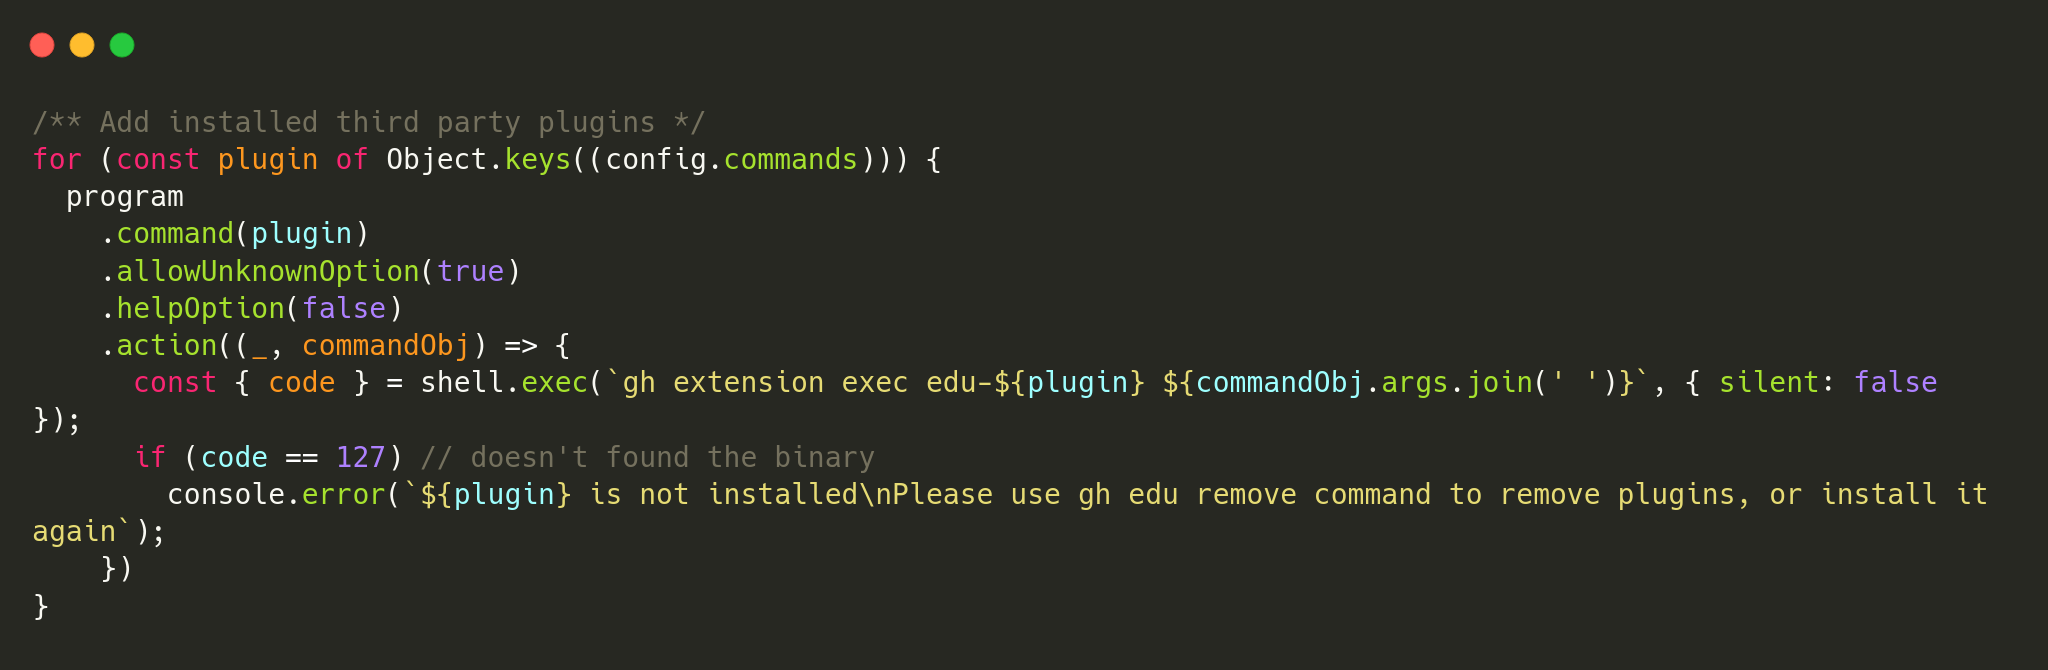
\includegraphics[width=\textwidth]{images/addThirdParty.png}}
%     \caption{Implementación. Controlador. Añadir extensiones third-party}
%     \label{fig:addThirdParty}
% \end{figure}

% Todas las extensiones, que se hayan instalado en el sistema a través de \verb|gh-edu|, se añadirán como comandos disponibles. También se activa la posibilidad de usar opciones desconocidas y se delega su gestión al subcomando en cuestión. Así mismo se desactiva la ayuda y en el manejo de errores solo se comprueba que el comando haya sido ejecutado, pues naturalmente de estas tareas se tiene que ocupar cada extensión.

% Aquí se deja ver la madurez del programa al permitirnos utilizar comandos desconocidos, función que, al momento de escribir estas líneas, todavía no es posible con \href{https://github.com/spf13/cobra/issues/739}{cobra}.

% \subsection{Manejo del único punto de información: data.json} \label{impl:data.json}
% Lo primero que el programa hace al ser ejecutado, es comprobar la validez del fichero. La siguiente figura (\ref{fig:dataGraph}) muestra los estados por los que se pasa para lograrlo.

% \begin{figure}[H]
%     \centering
%     \makebox[\textwidth][c]{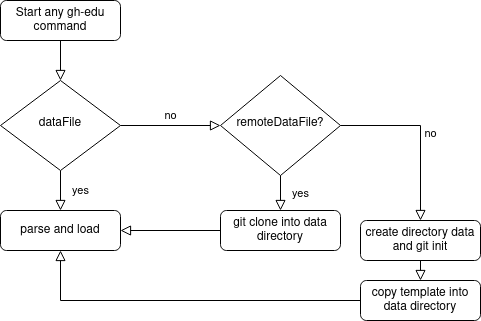
\includegraphics[width=0.5\textwidth]{images/createConfig.png}}
%     \caption{Obtención del archivo data.json}
%     \label{fig:dataGraph}
% \end{figure}

% Es primer paso es comprobar si se encuentra en la localización correspondiente (\verb|~/.config/gh-edu/data.json|). De no ser así, se intenta conseguirlo desde el repositorio \verb|gh-edu-profile|. Como última instancia se crea un fichero nuevo, partiendo de una plantilla que contiene todos los campos necesarios.

% Sabiendo que el fichero está disponible, pasamos a validar su contenido. Primero se \glspl{deserialization} para comprobar que es un fichero JSON válido. Acto seguido pasamos a realizar una comprobación simple de los campos, comprobando que estén en el fichero y que las \glspl{regex} sean válidas.

% \begin{figure}[H]
%     \centering
%     \makebox[\textwidth][c]{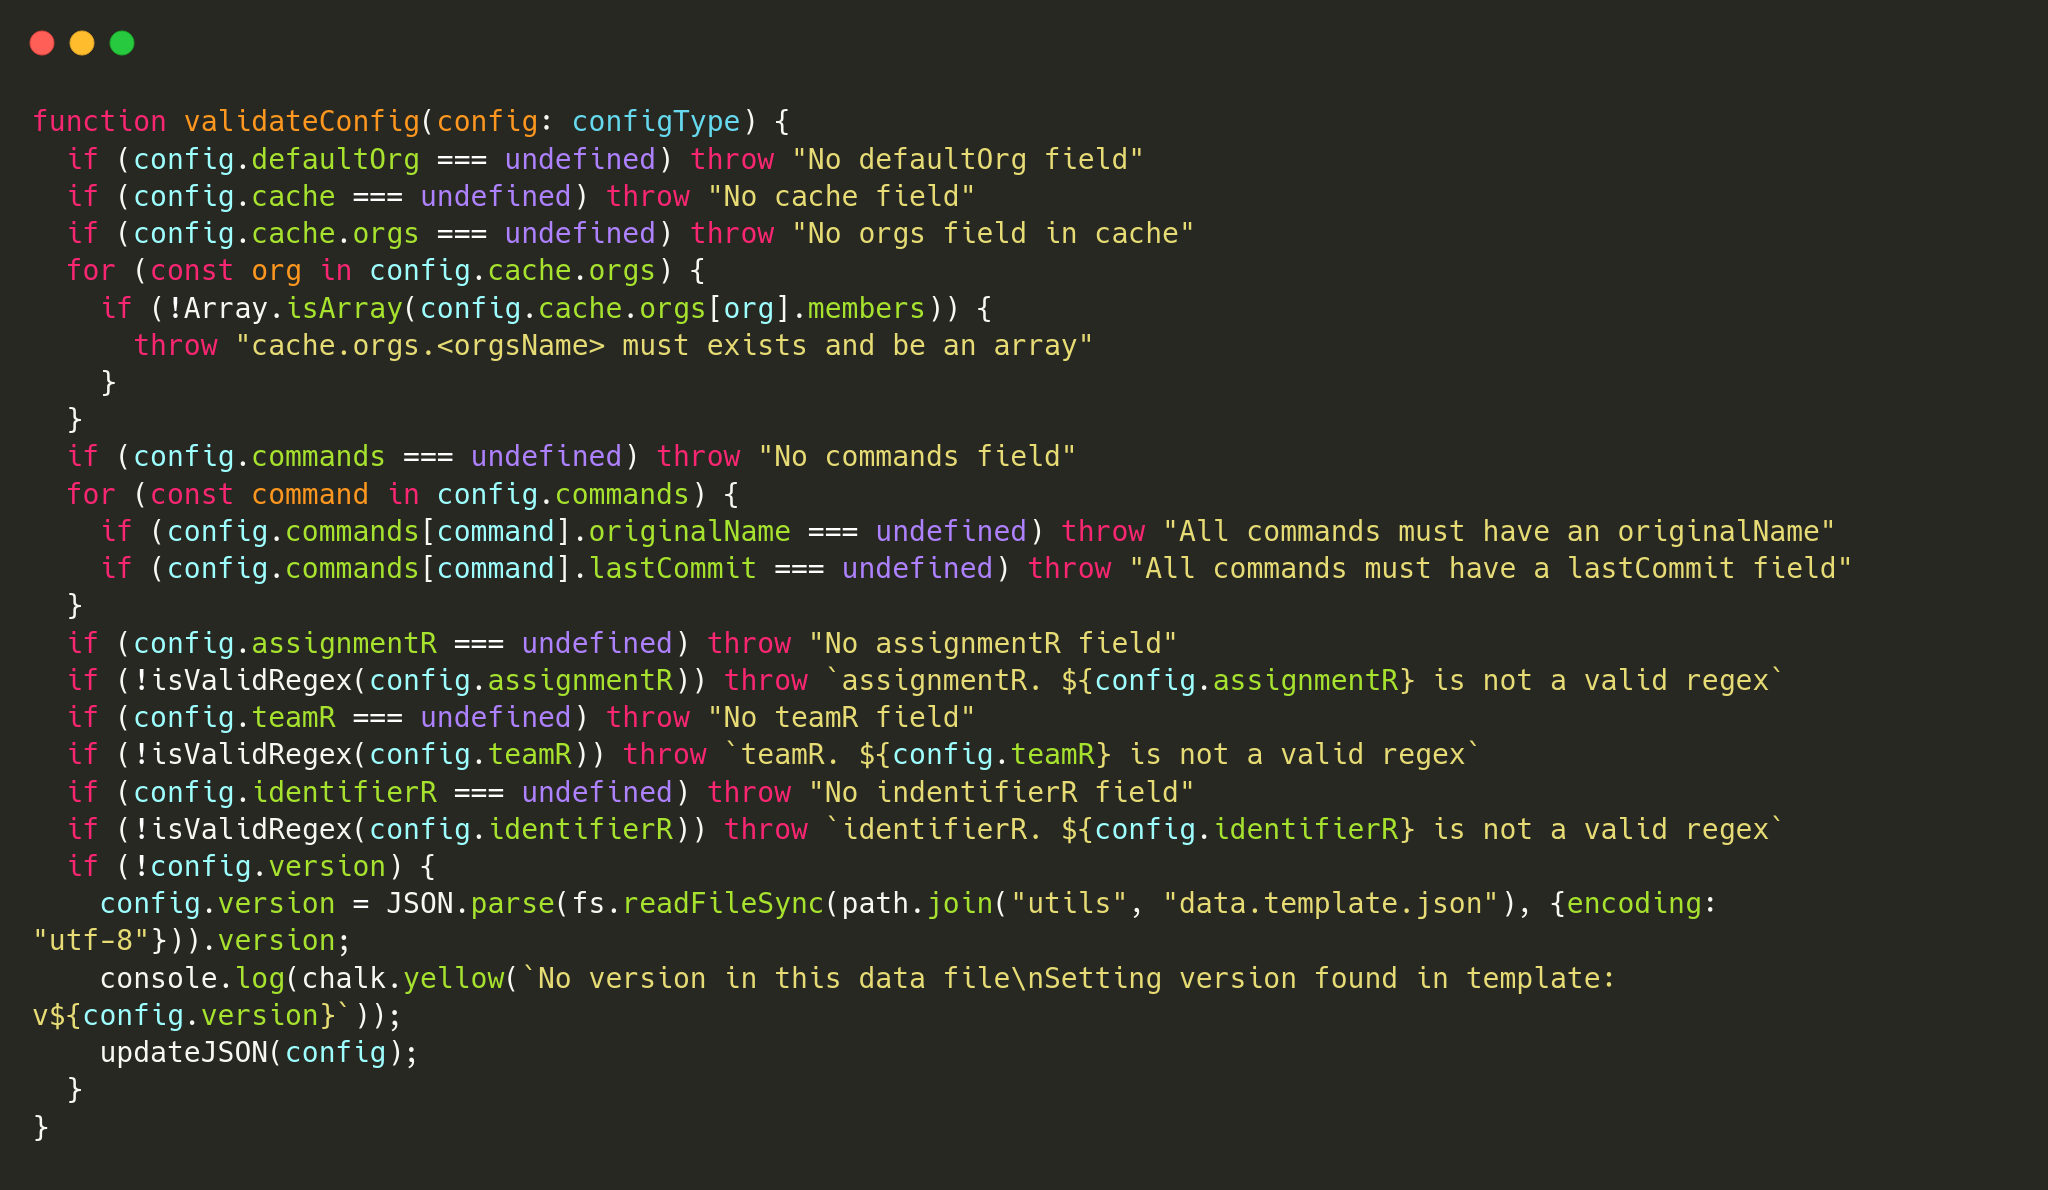
\includegraphics[width=\textwidth]{images/comprobacion.png}}
%     \caption{Implementación. data.json. Comprobamos que los campos son válidos}
%     \label{fig:comprobar}
% \end{figure}

% Cada vez que se quiera actualizar la información, se actualiza la variable donde se cargó el fichero, se \glspl{serialization} y se escribe de vuelta al fichero.

% \section{Extensión minimalista: {\tt gh-edu-view}}\label{sec:gh-edu-view-implementation}

% A la hora de escribir una extensión para \verb|gh-edu| en \verb|JS|, se procede de la misma forma que con una extensión \verb|gh|.
% Deben crearse los ficheros \verb|gh-edu-view/gh-edu-view| (script bash) y \verb|gh-edu-view/gh-edu-view.js| (programa \verb|JS|).

% Para intentar conseguir los identificadores relacionados a los alumnos, con nada más que la información proporcionada con GitHub, no nos queda otra opción que buscar en todos los campos, donde dicha información podría estar disponible, y devolver un \emph{array} con todos los posibles resultados.

% \begin{figure}[H]
%     \centering
%     \makebox[\textwidth][c]{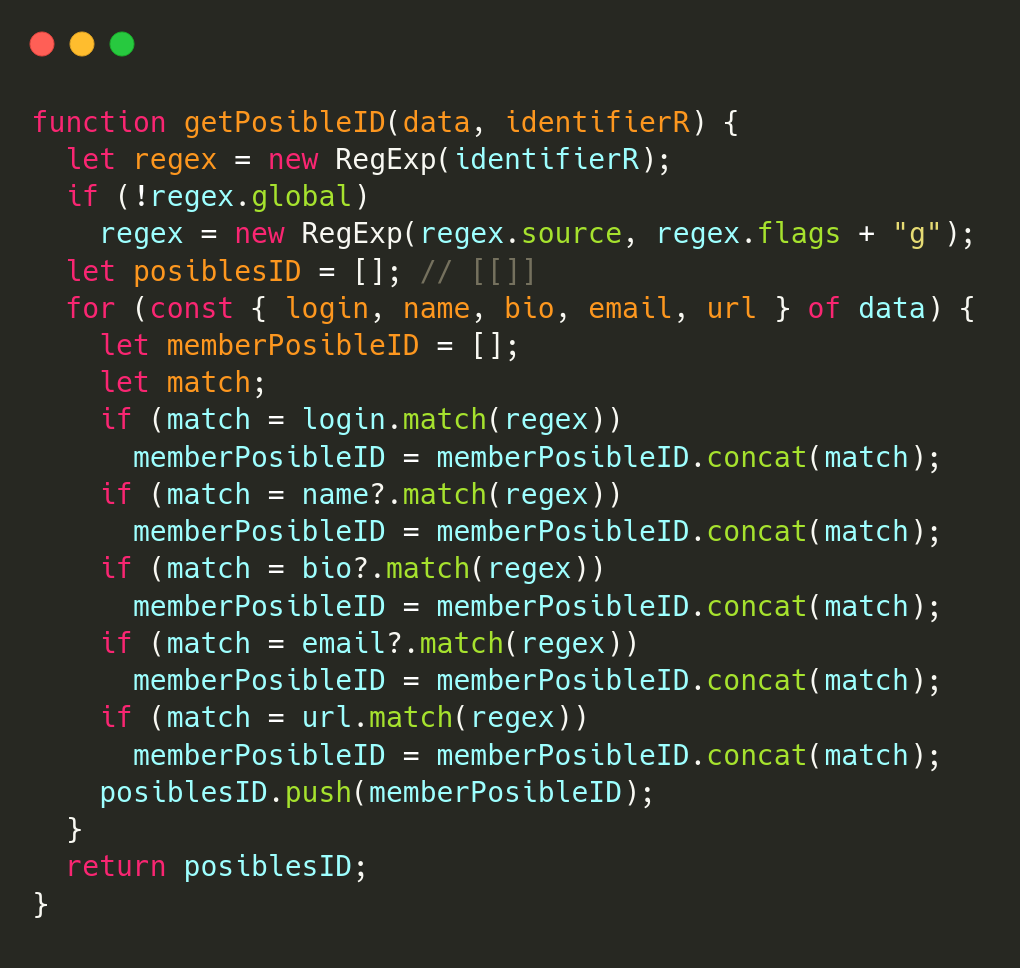
\includegraphics[width=0.5\textwidth]{images/posibleID.png}}
%     \caption{Implementación. gh-edu-view. Obtención de posibles identificadores}
%     \label{fig:viewId}
% \end{figure}

% Toda la información proporcionada por el comando \verb|members| se puede conseguir con una simple petición en GraphQL (figura \ref{fig:viewQuery}).

% \begin{figure}[H]
%     \centering
%     \makebox[\textwidth][c]{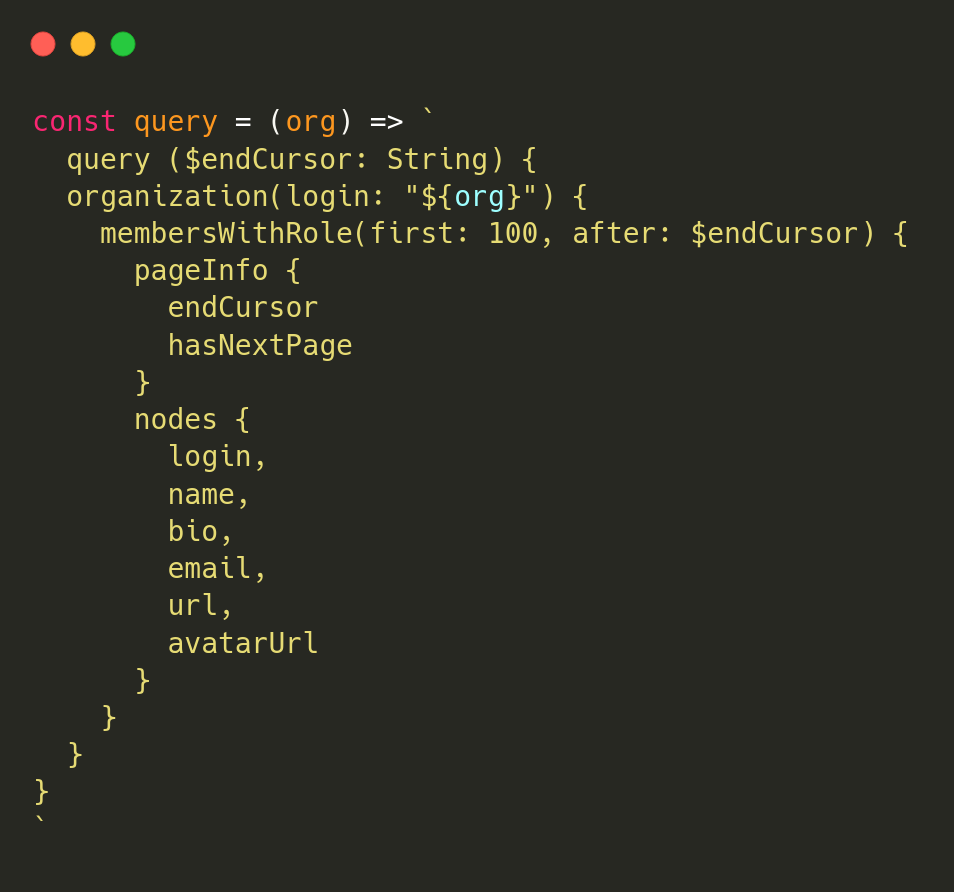
\includegraphics[width=0.5\textwidth]{images/view-query.png}}
%     \caption{Implementación. gh-edu-view. Petición para conseguir diversos campos de cada alumno}
%     \label{fig:viewQuery}
% \end{figure}

% \section{{La librería \tt shelljs} y el manejo de E/S: {\tt gh-edu-data}} \label{impl:gh-edu-data}
% Uno de los defectos de \verb|shelljs| que ya se ha comentado en el apartado de \textbf{Tecnologías} (\ref{shelljs}) es como no permite el uso de \verb|STDIN| o tuberías. Algo importante en este proyecto, pero especialmente en esta extensión por el uso avanzado de \verb|fzf| y \verb|jq|. Estas dos tecnologías, a pesar de ser completamente independientes la una a la otra, pueden trabajar conjuntamente gracias a su diseño flexible y minimalista a través de tuberías, haciendo posible la previsualización dinámica de los elementos en el comando \verb|log| (figura \ref{fig:interface-log})

% Este comportamiento es requerido, ya que no es posible pasar un objeto \verb|JS| o un \emph{array} al input de un programa que todavía no ha sido ejecutado. Solo se puede usar cadenas de texto. Lo ideal es ejecutar el comando, y de forma asíncrona ir procesando la estructura de datos, enviando cadenas de texto, como se hace en \verb|gh-edu-plagiarism| (gracias a \href{https://pkg.go.dev/os/exec@go1.18.3#Cmd.StdinPipe}{cmd.StdInPipe}).

% Hasta que la \href{https://github.com/shelljs/shelljs/issues/424}{incidencia 424} no sea resuelta, se ha tenido que realizar una solución alternativa utilizando ficheros temporales. La idea consiste en formatear el objeto o \verb|array| y escribir el resultado en un fichero, de esta forma podemos leer el fichero y transmitir esa información por medio de una tubería a otro comando en el mismo momento en el que se ejecuta el comando.

% \section{Concurrencia con Go y CSP: {\tt gh-edu-plagiarism}} \label{diseño:gh-edu-plagiarism}
% A diferencia del resto de extensiones \verb|plagiarism| está implementado en Go. Uno de los motivos del cambio de lenguaje es demostrar como se puede desarrollar extensiones en cualquier lenguaje sin muchas dificultades.

% También, como se comentó en \textbf{Tecnologías} (\ref{go}) este programa es altamente concurrente y paralelo. Go cuenta con un modelo de concurrencia bastante particular basado en el trabajo teórico de Tony Hoare \emph{Communicating Sequential processes} (CSP) \cite{hoare1985communicating}.

% Para entender las explicaciones de esta sección es necesario conocer dos conceptos: las gorutinas y los canales. Las gorutinas son \glspl{corrutine} independientes que se ejecutan en hilos verdes (\emph{green threads}), los cuales son hilos emulados generados en tiempo de ejecución, estos hilos se multiplexan a hilos reales del procesador a través del \verb|Go scheduler|, que determina cuanto tiempo debe estar cada hilo verde consumiendo CPU.

% Los canales son la estructura de datos que nos permite enviar información de una gorutina a otra y también sirven de elemento sincronizador, cuando se envía un elemento, la gorutina no continua hasta que el otro lado (el emisor) haya recibido la información y viceversa.

% La explicación de la figura \ref{fig:plagiarism} en términos de código sería la siguiente:\\
% Cada bloque dentro del módulo \verb|Concurrent| es una gorutina que se ejecuta de forma independiente y cada flecha pertenece a un canal, que sincroniza y a su vez transmite información de una gorutina a otra.

% La gorutina \verb|clone| va creando a su vez gorutinas a medida que más repositorios se vayan filtrando. Debido a que las gorutinas apenas consumen recursos, está bien eliminar y crear tantas como queramos. No obstante, como estamos realizando programación paralela, tenemos que tener cuidado de que no haya muchas más gorutinas corriendo que núcleos disponibles en el procesador, pues entonces conseguiríamos el efecto contrario al deseado, ralentizando toda la aplicación debido al constante cambio de contexto entre hilos. Para limitar la creación de gorutinas al número de núcleos disponibles se ha utilizado un semáforo. Un semáforo es una variable o estructura de datos que permite una cantidad arbitraria de procesos. Un semáforo binario es a efectos prácticos un \verb|lock| o \verb|mutex|.

% \begin{figure}[H]
%     \centering
%     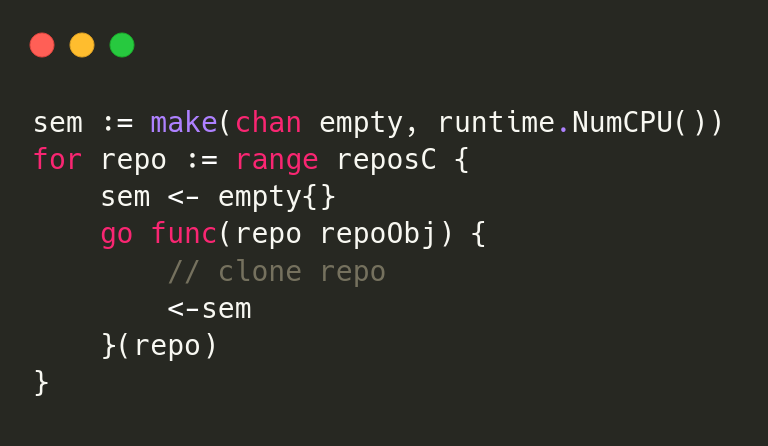
\includegraphics[width=0.5\linewidth]{images/concurrency-go.png}
%     \caption{Paralelismo limitado con un sémaforo}
%     \label{fig:concurrencyGo}
% \end{figure}
% El código que lo implementa (figura \ref{fig:concurrencyGo}) ha sido simplificado para explicar el funcionamiento del paralelismo y el semáforo.

% El canal \verb|sem| es un canal con buffer, esto quiere decir que no para el flujo (no sincroniza) hasta que el buffer se llene. El tamaño de dicho buffer es \verb|runtime.NumCPU()| que retorna el número de núcleos disponibles al ejecutar el programa. En cada iteración del bucle \verb|repo| contiene un nuevo repositorio proveniente del módulo \verb|Filter| y enviamos un elemento al canal \verb|sem|, el elemento en cuestión es irrelevante, estamos usando el canal por sus propiedades de sincronización, no para la transferencia de datos. Después ejecutamos una gorutina anónima que se encarga de clonar el repositorio, cuando termine escucha y descarta del canal \verb|sem|.

% De esta forma, si \verb|sem| está lleno significa que ya hay tantos procesos ejecutándose como núcleos hay disponibles, por lo que el programa queda en espera hasta que quede un hueco en el semáforo.

% % Esto va en diseño. Otro de los motivos por los cuales se eligió Go es que a la hora de diseñar la extensión me percate de que el programa sería altamente concurrente y paralelo. Uno de los motivos por los cuales se creó Go fue para poder aprovechar al máximo los varios núcleos que suele tener cualquier dispositivo moderno. Así, las instituciones educativas que reutilizan la misma organización para una misma asignatura a lo largo de varios años, y por ende tienen muchos repositorios y miembros, no verán su experiencia lastrada. También se tuvo en cuenta que Go tiene soporte de primera clase con \verb|gh| y uno de los casos de uso más comunes del lenguaje son aplicaciones CLI.

% \begin{figure}[H]
%     \centering
%     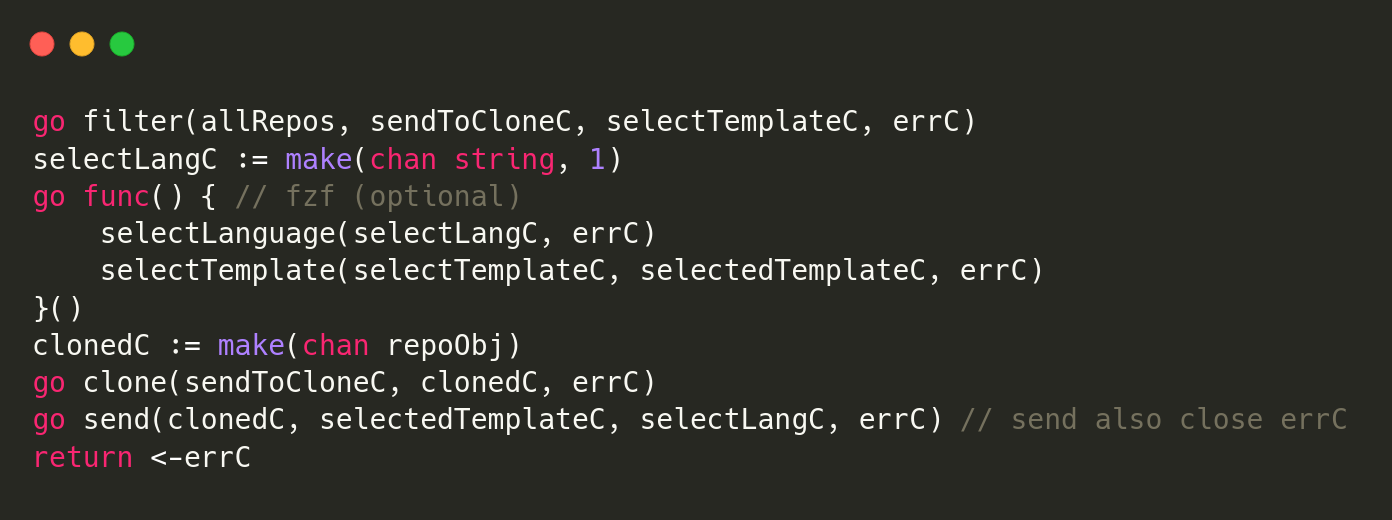
\includegraphics[width=\linewidth]{images/go-code.png}
%     \caption{Código general de plagiarism}
%     \label{fig:goCode}
% \end{figure}

 